% This is "sig-alternate.tex" V2.0 May 2012
% This file should be compiled with V2.5 of "sig-alternate.cls" May 2012
%
% This example file demonstrates the use of the 'sig-alternate.cls'
% V2.5 LaTeX2e document class file. It is for those submitting
% articles to ACM Conference Proceedings WHO DO NOT WISH TO
% STRICTLY ADHERE TO THE SIGS (PUBS-BOARD-ENDORSED) STYLE.
% The 'sig-alternate.cls' file will produce a similar-looking,
% albeit, 'tighter' paper resulting in, invariably, fewer pages.
%
% -% This is "sig-alternate.tex" V2.0 May 2012
% This file should be compiled with V2.5 of "sig-alternate.cls" May 2012
%
% This example file demonstrates the use of the 'sig-alternate.cls'
% V2.5 LaTeX2e document class file. It is for those submitting
% articles to ACM Conference Proceedings WHO DO NOT WISH TO
% STRICTLY ADHERE TO THE SIGS (PUBS-BOARD-ENDORSED) STYLE.
% The 'sig-alternate.cls' file will produce a similar-looking,
% albeit, 'tighter' paper resulting in, invariably, fewer pages.
%
% ----------------------------------------------------------------------------------------------------------------
% This .tex file (and associated .cls V2.5) produces:
%       1) The Permission Statement
%       2) The Conference (location) Info information
%       3) The Copyright Line with ACM data
%       4) NO page numbers
%
% as against the acm_proc_article-sp.cls file which
% DOES NOT produce 1) thru' 3) above.
%
% Using 'sig-alternate.cls' you have control, however, from within
% the source .tex file, over both the CopyrightYear
% (defaulted to 200X) and the ACM Copyright Data
% (defaulted to X-XXXXX-XX-X/XX/XX).
% e.g.
% \CopyrightYear{2007} will cause 2007 to appear in the copyright line.
% \crdata{0-12345-67-8/90/12} will cause 0-12345-67-8/90/12 to appear in the copyright line.
%
% ---------------------------------------------------------------------------------------------------------------
% This .tex source is an example which *does* use
% the .bib file (from which the .bbl file % is produced).
% REMEMBER HOWEVER: After having produced the .bbl file,
% and prior to final submission, you *NEED* to 'insert'
% your .bbl file into your source .tex file so as to provide
% ONE 'self-contained' source file.
%
% ================= IF YOU HAVE QUESTIONS =======================
% Questions regarding the SIGS styles, SIGS policies and
% procedures, Conferences etc. should be sent to
% Adrienne Griscti (griscti@acm.org)
%
% Technical questions _only_ to
% Gerald Murray (murray@hq.acm.org)
% ===============================================================
%
% For tracking purposes - this is V2.0 - May 2012

\documentclass{sig-alternate}
\usepackage{fixltx2e}
\usepackage{xcolor}
\usepackage{amsmath,array}
\usepackage{multirow}
\newcolumntype{L}[1]{>{\raggedright\arraybackslash}m{#1}}
\def\SPSB#1#2{\rlap{\textsuperscript{\textcolor{red}{#1}}}\SB{#2}}
\def\SP#1{\textsuperscript{\textcolor{black}{#1}}}
\def\SB#1{\textsubscript{\textcolor{black}{#1}}}
\newenvironment{myquote}
               {\list{}{\rightmargin   \leftmargin
                        \parsep        0in }%
                \item\relax}
               {\endlist}
\newcommand{\userquote}[2]{\begin{samepage}\begin{myquote} 
     \em{\small{#2\begin{flushright}---#1\end{flushright}}}
   \end{myquote}\end{samepage}}
%Quote code
%\newif\ifquoteopen
%\catcode`\"=\active % lets you define `"` as a macro
%\DeclareRobustCommand*{"}{%
%   \ifquoteopen
%     \quoteopenfalse ''%
%   \else
%     \quoteopentrue ``%
%   \fi
%}

%End of quote code

\begin{document}
\setlength{\parindent}{0pt}
\CopyrightYear{2016}
\setcopyright{acmcopyright}
\conferenceinfo{ACM DEV '16,}{Nov 18-21, 2016, Nairobi, Kenya}
%\isbn{978-1-4503-4306-0/16/06}\acmPrice{\$15.00}
%\doi{http://dx.doi.org/10.1145/2909609.2909664}
%
% --- Author Metadata here ---
%\conferenceinfo{ICTD'16}{June 3-6 2016, Ann Arbor, Michigan, USA}
%\CopyrightYear{2007} % Allows default copyright year (20XX) to be over-ridden - IF NEED BE.
%\crdata{0-12345-67-8/90/01}  % Allows default copyright data (0-89791-88-6/97/05) to be over-ridden - IF NEED BE.
% --- End of Author Metadata ---

%\title{Alternate {\ttlit ACM} SIG Proceedings Paper in LaTeX
%\title{Leveraging on Families' Social Interactions on Utilization of Personal Health Informatics through Intermediaries}
\title{A Family Wellness App: Engage Children to Manage Wellness of Adults}
%
% You need the command \numberofauthors to handle the 'placement
% and alignment' of the authors beneath the title.
%
% For aesthetic reasons, we recommend 'three authors at a time'
% i.e. three 'name/affiliation blocks' be placed beneath the title.
%
% NOTE: You are NOT restricted in how many 'rows' of
% "name/affiliations" may appear. We just ask that you restrict
% the number of 'columns' to three.
%
% Because of the available 'opening page real-estate'
% we ask you to refrain from putting more than six authors
% (two rows with three columns) beneath the article title.
% More than six makes the first-page appear very cluttered indeed.
%
% Use the \alignauthor commands to handle the names
% and affiliations for an 'aesthetic maximum' of six authors.
% Add names, affiliations, addresses for
% \additionalauthors command.
% These 'additional authors' will be output/set for you
% without further effort on your part as the last section in
% the body of your article BEFORE References or any Appendices.

\numberofauthors{3} %  in this sample file, there are a *total*
% of EIGHT authors. SIX appear on the 'first-page' (for formatting
% reasons) and the remaining two appear in the \additionalauthors section.
%
\author{
% You can go ahead and credit any number of authors here,
% e.g. one 'row of three' or two rows (consisting of one row of three
% and a second row of one, two or three).
%
% The command \alignauthor (no curly braces needed) should
% precede each author name, affiliation/snail-mail address and
% e-mail address. Additionally, tag each line of
% affiliation/address with \affaddr, and tag the
% e-mail address with \email.
%
% 1st. author
\alignauthor
        Ntwa Katule \\
        \affaddr{University of Cape Town}\\
        \affaddr{Department of Computer Science}\\
        \affaddr{Cape Town, South Africa}\\
        \email{katulentwa@gmail.com}
% 2nd. author
\alignauthor
Melissa Densmore\\
        \affaddr{University of Cape Town}\\
        \affaddr{Department of Computer Science}\\
        \affaddr{Cape Town, South Africa}\\
        %\affaddr{Institute for Clarity in Documentation}\\
        %\affaddr{P.O. Box 1212}\\
        %\affaddr{Dublin, Ohio 43017-6221}\\
        \email{mdensmore@cs.uct.ac.za}
% 3rd. author
\alignauthor Ulrike Rivett\\
        \affaddr{University of Cape Town}\\
        \affaddr{Department of Information Systems}\\
        \affaddr{Cape Town, South Africa}\\
        \email{ulrike.rivett@uct.ac.za}
       %\affaddr{The Th{\o}rv{\"a}ld Group}\\
        %\affaddr{1 Th{\o}rv{\"a}ld Circle}\\
        %\affaddr{Hekla, Iceland}\\
        %\email{larst@affiliation.org}
%\and  % use '\and' if you need 'another row' of author names
% 4th. author
%\alignauthor Lawrence P. Leipuner\\
%       \affaddr{Brookhaven Laboratories}\\
%       \affaddr{Brookhaven National Lab}\\
%       \affaddr{P.O. Box 5000}\\
%       \email{lleipuner@researchlabs.org}
% 5th. author
%\alignauthor Sean Fogarty\\
%       \affaddr{NASA Ames Research Center}\\
%       \affaddr{Moffett Field}\\
%       \affaddr{California 94035}\\
%       \email{fogartys@amesres.org}
% 6th. author
%\alignauthor Charles Palmer\\
%       \affaddr{Palmer Research Laboratories}\\
%       \affaddr{8600 Datapoint Drive}\\
%       \affaddr{San Antonio, Texas 78229}\\
%       \email{cpalmer@prl.com}
}
% There's nothing stopping you putting the seventh, eighth, etc.
% author on the opening page (as the 'third row') but we ask,
% for aesthetic reasons that you place these 'additional authors'
% in the \additional authors block, viz.
%\additionalauthors{Additional authors: John Smith (The Th{\o}rv{\"a}ld Group,
%email: {\texttt{jsmith@affiliation.org}}) and Julius P.~Kumquat
%(The Kumquat Consortium, email: {\texttt{jpkumquat@consortium.net}}).}
\date{30 July 1999}
% Just remember to make sure that the TOTAL number of authors
% is the number that will appear on the first page PLUS the
% number that will appear in the \additionalauthors section.

\maketitle 

\begin{abstract} 
The pandemic of lifestyle-related chronic diseases has led to an advent of personal health informatics, with the goal of persuading individuals to adopt healthful lifestyles. Such systems implement various motivational affordances to promote ongoing use. Design of such systems focuses in engaging only the beneficiary of information derived from those systems. In this study we explored how one can use gamification to motivate ongoing usage of such systems in the context of intermediated technology use. We studied the effect of gamification in motivating young family members in assisting adults who might be less conversant or intimidated with such a technology. We compared two designs of a mobile wellness application of which one prototype was gamified and the other one was not gamified. Our findings suggest that virtual rewards can enhance usage of such systems through intermediary users. We highlight some of the design implications in order to foster perceived enjoyment in using such a system.    
\end{abstract}
%
% The code below should be generated by the tool at
% http://dl.acm.org/ccs.cfm
% Please copy and paste the code instead of the example below. 
%

\begin{CCSXML}
<ccs2012>
<concept>
<concept_id>10002944.10011122.10002947</concept_id>
<concept_desc>General and reference~General conference proceedings</concept_desc>
<concept_significance>500</concept_significance>
</concept>
<concept>
<concept_id>10003120.10003121.10011748</concept_id>
<concept_desc>Human-centered computing~Empirical studies in HCI</concept_desc>
<concept_significance>300</concept_significance>
</concept>
<concept>
<concept_id>10003456.10010927</concept_id>
<concept_desc>Social and professional topics~User characteristics</concept_desc>
<concept_significance>100</concept_significance>
</concept>
</ccs2012>
\end{CCSXML}

\ccsdesc[500]{General and reference~General conference proceedings}
\ccsdesc[300]{Human-centered computing~Empirical studies in HCI}
\ccsdesc[100]{Social and professional topics~User characteristics}

%
% End generated code
%

%
%  Use this command to print the description
%
\printccsdesc


%A category including the fourth, optional field follows...
\keywords{HCI4D, intermediated interactions, persuasive technologies, gamification, personal informatics, motivational affordances, health}

\section{Introduction} 
Lifestyle-related diseases are now attracting many players seeking to design low cost and tailored information and communications technology (ICT)- based systems for supporting lifestyle change and disease management\cite{arsand:mobile} with most recent development focusing in persuasive technlogies. A systematic review of 95 studies on persuasive technologies found out that persuasive systems have the capability to persuade because their design include implementation of persuasion stimuli \cite{hamari2014persuasive}.\newline
Persuasive systems include personal informatics which can be used for persuasion of health behaviours. Personal informatics systems are interactive applications that support users to become self-aware of patterns in the behaviours, by providing means to collect personal history, as well as tools for its review or analysis \cite{li2011:personal,li2012:personal}. Persuasion stimuli in a personal informatics rely on their ability to support reflective learning/self-reflection \cite{li2011:understanding}. Reflective learning entails reviewing of collected personal data to learn about oneself and the user always alternates between two phases known as discovery of a behaviour pattern and maintenance of a better behaviour\cite{li2011:understanding}. These phases are usually supported through feedback mechanisms such as bar charts or other affective mechanisms such as gardens that represent steps walked (i.e Ubifit\cite{klasnja2009:using}) or Fish growing or shrinking depending to an increase or decrease in the number of steps walked (i.e Fish'nSteps \cite{lin2006:fish}). The aforementioned techniques can further be supplemented with social comparison\cite{Oinas-kukkonen:psd} or competitions with others \cite{comber2013:designing} in some systems. General approaches on how to design such systems have been proposed with ideas coming from both HCI\cite{li2010:stage} and persuasive technologies fields \cite{fogg2009:behavior,Oinas-kukkonen:psd,Oinas-Kukkonen:foundation}.  \newline
However utilization of such systems may be constrained to specific demographics such as young or experienced users of technology. For instance , one study evaluated two of the popular fitness apps, Nike+ and RunKeeper, and concluded that the two apps are not ready to accommodate older adults needs \cite{silva2014:smartphones}. In addition to that, in developing countries there are scenarios of intermediated technology use for users who are inexperience or intimidated by technology and many of the existing apps are designed to accommodate only direct users of technology \cite{sambasivan2010}. Therefore, in personal health informatics, features that foster ongoing use are targeted towards beneficiaries of the information processed by the app. But in the context of intermediated technology there is an intermediary user who is there to facilitate access of information to beneficiary users hence that facilitator needs to also be motivated to support ongoing use of a personal health informatics.\newline
In our work, we replicate the idea of intermediated technology use into personal health informatics as we believe that it can support users who are less conversant in technology. Instead of just involving an adult beneficiary user in interacting with a personal health informatics, we bring young family members to become part of the interaction process and apply gamification to foster ongoing use. One study found out that perceived interest to use gamification decreases with age and this implies that such a gamified system might be more effective if utilized through younger populations\cite{v2014motivational}.\newline
In this study we report on the outcome of using gamification and how different it is in comparison to involving intermediaries without gamification. We also propose approaches that can enhance the impact of gamification in the context of personal health informatics used through intermediary users.
\section{Related Work} 
The roots of gamification come from games. Gamification is an idyllic avenue that is used in engaging users with personal informatics or persuasive technology targeting health behaviour change because of its ability to trigger intrinsic experiences \cite{hamari2014persuasive}. Gamification borrows game design mechanics such as points, leader-boards, badges, etc in non-game contexts\cite{deterding2011game}. It brings together the motivation pull from video games. Gamification has been found to have a potential to address motivational mechanisms and thereby fosters motivation \cite{sailer2013:psychological}. The motivational  factors of gamification can be explained using a self-determination theory on the next sub-section.    
\subsection{Overview of Self-Determination Theory}
Self-determination theory (SDT)\cite{deci1985:intrinsic} is a well established theory of motivation that explains why people choose to engage or disengage on various activities. The choice depends on social conditions of which people develop and function, of whereby these conditions mediate of whether people will become interested with certain activities or lose interest on those activities. SDT research has been focusing on social conditions that positively or negatively affect the natural process of motivation, and health psychological development\cite{ryan2000:self}. SDT postulates the extent to which a behaviour is internally self-regulated and how one can apply external rewards to increase internal self-regulation of a behaviour \cite{ryan2000:self}. This process of transmuting an externally rewarded activity to intrinsically motivated activity is called internalization. Since behaviours can be influenced by social conditions, then it means at one point a behaviour that was once externally motivated can become internalized.\newline
An assumption from SDT is that people have tendencies of naturally being motivated by integrating their social and physical world to self-regulation of behaviours \cite{lee2015:relating}. Underlying the core of SDT, there are two sub-theories namely cognitive evaluation theory and organismic integration theory \cite{ryan2000:self}. The former explains about social factors that drive intrinsic motivation of a behaviour. The latter focuses on external factors that can harm or foster intrinsic motivation.\newline  
Within the cognitive evaluation theory, SDT suggests the basic psychological needs for a behaviour to become intrinsically motivated and these are (1) autonomy; (2) competence; (3) relatedness \cite{deci1985:intrinsic}.\newline
The following explanation of the three basic psychological need is based on these sources (\cite{deci1985:intrinsic,ryan2000:self,lee2015:relating}). Autonomy is freedom to self-initiate and regular a behaviour. Autonomy emphasizes on the importance of individual's ability to choose their own way of presenting oneself without peer pressure. With autonomy people can uniquely choose an identify to represent oneself. Autonomy gives individual freedom to choose when and how they want to initiate a behaviour. Competence emphasizes the need for individuals to be presented with challenges that give individual a chance to sharpen their skills in order to match those challenges. This is process is appropriate for ones' health psychological development and  overall well-being. Relatedness is the desire by individuals to feel a sense of belongingness. People like to be connected to others. \newline  
SDT postulates that external rewards that support the three aforementioned psychological needs can foster internalization of a behaviour, however, there is a caveat on introducing external rewards to an already intrinsically motivated behaviour because external rewards can harm intrinsic motivation \cite{ryan2000:self}.\newline
Organismic integration theory explains the process of internalizing a behaviour through external rewards. External rewards are classified as follows, \emph{external, introjected, identified, and integrated regulations} \cite{ryan2000:self,lee2015:relating}. In external regulation, the causality of  regulation of behaviour is coming from outside. This can monetary rewards or other forms of rewards, while,in external rewards, individuals self-regulate a behaviour but they don't fully integrate it as their own therefore it continues to depend on rewards.\cite {lee2015:relating}. In identified  regulations, individuals have accepted a behaviour and its regulation by putting value to a behaviour, while in integrated regulation,  a behaviour is fully integrated ones sense of values \cite{lee2015:relating}.\newline 
SDT is very powerful as it can explain motivational factors from myriad of domains such as gaming\cite{ryan2006:motivationalpull}, physical activity\cite{power2011:obesity}, tobacco cessation\cite{williams2006:testing}, energy saving \cite{webb2013:self}, etc. In the next sub-section it is explained how SDT fits within user experience and its relation to gamification.  
\subsection{SDT in User Experience and Gamification}
One study emphasized on the importance of fulfilling six of the ten human needs such as, autonomy, relatedness, competence, , stimulation,  influence and security when using interactive products and media in order to improve user experience \cite{wiklund2009:needs}. The first three human needs are the core of self-determination theory. Partala and Kallinen evaluated most satisfying and unsatisfying user experiences in terms of experienced emotions, psychological needs (from SDT), and contextual factors and found out that the feeling of autonomy and competence to be the most satisfying user experience, and these two were never reported in the unsatisfying experiences category \cite{partala2012:understanding} .\newline 
The idea of user experience is now expanding motivational affordances. Zhang et al.\cite{zhang2008:motivational} suggested a list of motivational affordances that could be implemented in a system in order to foster its usage such as: (1) the system should afford self-identity and autonomy;(2) the system should support provision of challenges/competitions; (3)the system should allow users to relate to each other; etc. Different theoretical framework for user engagement have developed with an inspiration from SDT. Majority of these frame works explains how the concept of motivational affordances can be understood in the context of gamification. Deterding \cite{deterding2011:situated} developed  a conceptual model for situated motivational affordances of game elements that inspired by SDT. Nicholson proposed a framework for meaningful gamification and emphasized on integration of these four core concepts through user centred design; (1) organismic integration theory (sub theory of SDT); (2) situational relevance and situated motivational affordance; (2) universal design for learning; (3) player generated content . The aforementioned literatures suggest the potential of gamification in assimilating the concepts from SDT to enhance user experience.\newline 
Deterding et al. \cite{deterding2011game} situated work in gamification relative to similar initiatives in HCI and game studies which go back as far as early 1980s. This work suggest gamification brings gameful experiences and where gamification can be view as a game depends on the context of users but in a gameful experience there is the experiential
``flicker'' between gameful, playful, and other modes of experience and engagement. Since the goal of gamification is different from games, recent literature  tends to consider gamification more of a user experience rather than a gameful experience\cite{seaborn2015:gamification}. In the section we provide an overview of gamification in personal health informatics.
\subsection{Characteristics of Gamification Users}
Since gamification borrows its design elements from games, it is important to understand types of users in gamification to appropriately tailor a gamification intervention. For instance in online games there are three main components which are of users' interests, achievement, social, and immersion components, and interest in any of these features is determined by demographic information such as age, gender, etc \cite{yee2006:motivations}. There users who are interested with socializing more than anything else, or there will be users who are interested in achievements etc. Orji et al also \cite{orji2013:tailoring} emphasized tailoring of persuasive games targeting health to gamer type. Another study found out that players/users with high ``Game Identity Strength'' (GIS)- the degree in which players define gaming as part of the social identity, reported higher competence, autonomy, and relatedness, and in addition these hardcore players reported higher levels of persistence in playing compared to heavy and casual players \cite{neys2014:exploring}. In our work we didn't focus much on these aspects of gamer types but we point out some of the findings that exhibit these characteristics of gamer types. 
\subsection{Personal Health Apps and Gamification}  
One of the first apps to be published in HCI literature is \emph{``\textbf{Fish'n'Steps}''} \cite{lin2006:fish}. This apps was designed like a game. within the app there  was a fish bowl of where the fish gets excited depending on the level of activity of the user. This app presented social cues that made its users respond to it as if it was a physical being. For instance there were cases of were the fish was about die because of the user being inactive. This triggered an emotional response of sadness from the user.\newline
Another app was \emph{``\textbf{Ubifit}''} \cite{klasnja2009:using}. In this there was a garden that represents accumulation of physical activity. A garden could consist of flowers of different types which represent various activities such as cardio etc. This information was collected through an activity sensor and transmitted to a mobile phone of where a user would document an exercise type. The garden was being displayed as a screen saver. This kind of display is known as ambient display.\newline
Arteaga \cite{arteaga2010:persuasive} also presents a mobile persuasive application for to motivate kids with loss weight issues.The application is designed with games that allow users to select the game they want to play according to their personality. Another mHealth diabetes app namely \emph{``\textbf{bant}''} that uses gamification incentives showed an improvement in the frequency of blood glucose monitoring in adolescents with type 1 diabetes.\newline
Most of these apps have been implemented with motivational affordances to motivate a beneficiary user alone hence it is challenging to motivate ongoing use in the context where a beneficiary user has to to rely on an intermediary user to interact with his/her personal data. The phenomenon of young people providing support to adults on technological related problems is quite prevalent in both HCI and ICTD literature. Studies have explored factors influencing help-seeking and giving behaviours and have pointed out factors such group orientations towards tasks unfamiliarity with technology, social rapport,reciprocal benefits, the sense of being accountable and many others to play a significant role in mediating help-seeking and help giving behaviors in various contexts.\cite{sambasivan2010,poole:chh,kiesler:twi,parikh2006}. However the aforementioned literature in intermediated technology use is limited to general use of technology and it has not focused on specialized technology such as a personal health informatics which has received a lot of attention within HCI community. In our work, we designed a system that  utilizes gamification to motivate an intermediary user and a beneficiary user to work together to sustain ongoing use of the system.\newline 
The use of gamification has been studied in tasks such as image annotation\cite{mekler2013:points,mekler2013:disassembling},crowd reporting\cite{crowley2012:gamification}, data collection \cite{cechanowicz2013:effects} etc. and not in intermediated information tasks. The intermediated information task in our context is different as it more complex than the aforementioned tasks as there may be two users collaborating to engage with a user interface with the goal of one user assisting another user with his/her information needs. In this context an intermediary  user might be a passive user of health information and a beneficiary user is a recipient/beneficiary of health information. Motivational affordances need to motivate the two users to work together in engaging with the system.\newline
Our main research question attempts to understand the effectiveness of gamification in facilitating usage through intermediary users.
\section{Methods}
\subsection{Participants' Demography}
Participants for this study were recruited from Langa and Athlone, two of the many townships in Cape Town, South Africa. Majority of the households in these two townships fall under the bracket of low income earners in South Africa. The recruitment was facilitated one research assistant and her field work who reside in Langa and Athlone respectively.\newline
A total of fourteen adult participants were recruited with mean age of 44.21 years(S.D of 9.99 years). The youngest adult was 26 years of age while the oldest was 60 years of age. Thirteen of these adult participants were females. Each adult participant elected one of their children/grand children to work with. The two members of a pair were required to work together in using the ``Family Wellness App'' to self-monitor the wellness of an adult member of a pair (a beneficiary). The average age of children participants was 15.42 (S.D=2.06) years. The youngest intermediary participants was 12 years of age while the oldest was 20 years of age. The number of females and males intermediary participants were equal. Prior to be part of the study all adult participant signed consent forms and also all children participant sign an assent form which was also signed by their respective adult participants.\newline 
This is a justification why we selected kids who are family members. Perceived interest/enjoyment in gamification tends to diminish with increasing in age \cite{v2014motivational} and this suggests that young people are the perfect choice for intermediaries. We limited selection of intermediary users to family members because in our previous study we observed that familial relationships were the key to the success of such an intervention.  
\subsection{Experiment Design}
\begin{figure}
\centering
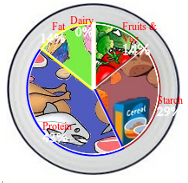
\epsfig{file=logbookapp.png, height=1.5in, width=3in}
\caption{Screen-shots showing logbook features: step bar chart and meal pie chart}
\label{figure:logbookapp}
\end{figure}
\begin{figure}
\centering
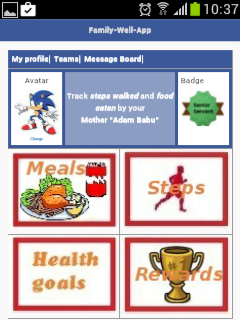
\epsfig{file=gameapp.png, height=1.5in, width=3in}
\caption{Screen-shots showing badges and a fitness garden}
\label{figure:gameapp}
\end{figure}
We were comparing two versions of the ``Family Wellness App''. The first version of the application was simply a logbook or journal (Figure \ref{figure:logbookapp}) that allows each pair of participants to view steps graphs and recording and viewing summaries of nutrition components of food consumed by a beneficiary within a pair. The second version also contained all the aforementioned features of logbook with an added gamification component (Figure \ref{figure:gameapp}). A gamification component consisted of a leader board (points' score board), badges,avatars, message board, botanical gardens, and fish tanks (aquarium). The rewards are earned by efforts in usage of the app, number of recorded meals consumed by a beneficiary participants (and what is the percentage of fruits and vegetables in those ,meals), and number of steps walked by a beneficiary participant. For instance  number and size of a fish might be determine by both usage of the app and a badge of which itself depends on steps.\newline
Both versions of the systems implemented reminders. In the logbook version, SMS were sent to remind intermediary participants to assist their respective beneficiary participants in self-monitoring of their steps and diet. In addition, those logbook reminders consisted of the current average number of steps walked per day by a beneficiary participant since the first day of using the app. In the gamified version, SMS were sent to remind pairs what they need to do in order to achieve rewards, and also what they have done so far (current status), and what remains to be done in order to attain a much higher status. For instance children can be reminded that recording more fruits and vegetable from their parents will give them a better botanical garden.\newline    
In order to compare the two versions of the system, the experimental design was within group which uses the same group of participants to test both system: (1)logbook only; and (2) the one that includes both logbook and gamified components. In order to minimize the impact of the learning effect on one experimental condition,each pair of participant was randomly assigned to one of the two experimental sequences. The first sequence consisted of individual pairs of participants that started with the logbook version and finished with the gamified version. This sequence is referred to as ``LG'' group. The second sequence  consisted of individual pairs of participants that started with the gamified version and finished with the logbook version. This sequence is referred to as ``GL'' group. A total of seven pairs of participants were assigned to the LG group while the remaining seven pairs were assigned to the GL group. 
\subsection{Data collection and analysis} 
Prior to data collection each intermediary participant from the 14 pairs was given an android phone that they could use with their adult participants. The phone were supposed to be handled by adults. Therefore kids were given phones to hand over them to their respective adults. A phone consisted of a native link to a web app and a native pedometer app.  Each pair of participants was allocated 1.3 GB of data to use through the duration of experiments. In addition each beneficiary participant was given a total of ZAR 240 (approx. US \$20) as a compensation for transport and their time for the duration of the study.\newline
We carried out this evaluation for a period of six weeks starting from Mid October 2015 running up to the last week of November 2015. The first four weeks were spent on logbook version for the ``LG'' group and  gamified version for the ``GL'' group. Thereafter, pairs in LG group were switched to gamified version while pairs in ``GL'' group were switched to logbook. Both versions of the app were used for two weeks after the aforementioned switching. The explanation of why four weeks in phase 1 and two weeks phase 2 is based on two reasons. Our plan was to divide time equally in three(3) weeks intervals. But phase one had extended to four(4) weeks instead of the three(3) weeks we had initially plan for and this was because we couldn't schedule a midline assessment immediately after the end of the third week since participants were not available. Therefore we couldn't do experimental switching before administering the questionnaire. We also couldn't extend the experimental period in phase two to have the same number of days as phase 1 because it was approaching December and it was going to be tricky to gather participants as some would have travelled for holidays. In order to address this problem of inequality, when we assess usage we only use a relative amount with respect to the number of days in which participants were given access to a particular experimental condition. This has not effect on either motivation to use any experimental condition since both logbook and gamification were both present in both phases. There the effects on motivations due to different durations are expect to cancel each other.\newline
We collected data through triangulation of usage logs for the two versions of the prototype,intrinsic motivation inventory(IMI) questionnaires, and interviews. We developed the IMI questionnaires with guidance of materials found on a ``Self-Determination Theory''\footnote{http://www.selfdeterminationtheory.org/intrinsic-motivation-inventory/} website which is maintained by researchers working on the theory including Richard Ryan and Edward Deci\cite{deci1985intrinsic} whom were early pioneers in developing the theory. These questionnaires were pretested in one of our early pilot studies.\newline
There were two sets of questionnaires, one for adult (beneficiaries) participants , and another one for children (intermediaries)  participants. Both questionnaires were administered at three points: (1) baseline (before experiments); (2) midline (the fourth week, before switching of experimental conditions; (3) endline (after concluding usage experiment at the end of the sixth week).\newline
The baseline questionnaire for the intermediary participants assesses the perceived enjoyment of intermediaries in helping other people with cellphone related tasks. The midline questionnaire for the intermediary participants assesses the ability of the two prototype to support the three basic psychological needs postulated by the self-determination theory: (1) autonomy, (2) competence, and (3) relatedness. Therefore we selected three sub-scales from the IMI questionnaire and these were (1)perceived autonomy, (2) perceived competence, and (3) perceived relatedness. The endline questionnaire for intermediaries was the same as the midline one.\newline
The baseline questionnaire for beneficiary assesses the the overall average IMI scores for: (1)self-monitoring of diet; (2)self-monitoring of activity. The IMI questionnaire included the following sub-scales;perceived competence, perceived autonomy, perceived relatedness, perceived enjoyment, perceived important, and perceived usefulness. The midline and endline questionnaire include the same baseline questionnaire. In addition, we assesses beneficiaries' perceived usefulness in using the family wellness app at midline and endline.\newline
Usage was measured by counting number of sessions and number of clicks. On comparison of usage of the two experiments we used number of sessions. The beginning of a new session was defined as a continuous period of time where an end user interacts with the app without interruptions. This period is whereby there is user's activities detected on the app while there were no user activities for the past one hour. If delay between activities is less than one hour it is then assumed that the last session is still active. If a user comes back after one hour has elapsed since the last detected user's activity then it is assumed they went away from the app and now they are coming back for a new session. 
This analysis excluded four pairs of users because they had various technical problems that hindered their full participation in both experimental conditions. The list of pairs that were excluded and reasons for their exclusion are summarised on Table \ref{table:usageproblems}.We compared usage by counting the number of sessions from each experimental condition. We computed the relative number of sessions since the number of days on which pairs of users spent on a particular experimental condition differ between LG and GL group. For instance the LG group spent nearly four weeks in logbook and two weeks in gamification while the GL group spent four weeks in gamification and two weeks in logbook. Therefore, we use number of session per day which is obtained using Equation \ref{equation:sessions}.\newline
\begin{table}[h!]
  \begin{center}
    \caption{Pairs with usability/technical problems that hinder their participation}
    \label{table:usageproblems}
	\begin{tabular}{|L{0.1cm}|p{1cm}|p{1.5cm}|p{4cm}|}
		\hline
		&Pair&Sequence&Problem\\
		\hline
		1&Pair A&GL group &App not loading due to poor Internet signal\\
		\hline
		2&Pair B&GL group& Miss-allocation of data bundles  \\
		\hline
		3&Pair C & LG group.& Pedometer never transmitted data to the server.\\
		\hline
		4&Pair D & LG group.& Pedometer stopped transmitting data to the server during the fourth week.\\
	\hline
	\end{tabular}
  \end{center}
\end{table}
\begin{equation}
\label{equation:sessions}
y=t\SB{i n}/d\SB{i n}
\end{equation} \newline
where:\newline
\emph{y} is number of sessions per day\newline
\emph{t\SB{n i}} is total number of sessions for pair ``n'' in experimental condition ``i''\newline
\emph{d\SB{n i}} is total number of days on which experimental condition ``i'' was available for pair ``n''.\newline
For instance, suppose pair one is from a LG group. This means they had  a logbook system for 27 days and a gamified system for 14 days. Suppose the number of sessions in logbook was 50 and the number of sessions in Gamified system was 30 then the relative number of sessions per day spent on logbook is going to be ``\textbf{50} divide by \textbf{27} days'' and the relative number of sessions spent on  a gamified system is going to be ``\textbf{30} divide by \textbf{27}.\newline
\section{Findings}
On this findings section we report first report on the general use of the app, secondly we report on the impact of the two versions of the app in satisfying intermediaries intrinsic motivation needs through fulfilment of the three basic psychological needs. The third outcome we explore if beneficiaries find the app to be useful for their health. And the fourth and the last outcome is the impact of the versions of the app in self-monitoring of diet and activity.\newline
\subsection{Usage Trend} 
The experimental duration was 27 days in the for both GL and LG groups in phase 1, 14 days  for both``LG' and ``GL'' groups in phase 2. Therefore, the sum is 41 days (6 weeks). In this period of six weeks, the average utilization of the app regardless of experimental conditions was 10.5 (SD=7.39) days. The most active usage was from a pair that utilized the app for a total of 26 days while the less active usage was from a pair that had used the app for only two days out of 41 days.\newline
\begin{figure}[htbp]
  \centering
    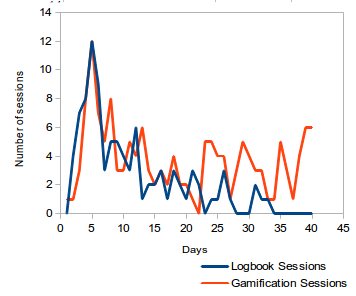
\includegraphics[width=0.3\textwidth]{scatter_daily_sessions.png}
    \rule{26em}{0.5pt}
  \caption{Total daily number of sessions from the two experimental conditions.}
  \label{figure:usagedailysessions}
\end{figure}\newline
\begin{table}[h!]
  \begin{center}
    \caption{Daily usage comparison between Logbook and Gamified systems for 41 days}
    \label{table:usagedays}
	\begin{tabular}{|L{4cm}|c|L{1.2cm}|L{1cm}|}
		\hline
		Groups&N&Rank Average&Sum Ranks\\
		\hline
   		Daily logbook sessions&41&33.72&1701.5\\
   		\hline 
   		 		    Daily gamification sessions&41&49.28& 1701.5\\
\hline
    \multicolumn{4}{|c|}{U=1159.5; Z=-2.9538; p=0.00318}\\
  \hline
	\end{tabular}
  \end{center}
\end{table}
\newline 
The differences on number of sessions per day didn't have a normal distribution shape. In order to get a normal distirbution shape of the differences, data was transformed using the natural log equation \ref{equation:log}. The differences between transformed logbook and gamification data had normal distribution shape. We performed a paired t test on the transformed data and the results showed that the Log mean of number of sessions per day was significantly higher on gamification condition when compared to logbook condition as shown on Table \ref{table:usagewellness2s}. What this finding suggests is that there was an indication of a significant increase in frequency of daily usage when pairs where in gamification condition.\newline
\begin{equation}
\label{equation:log}
y=log (x+1)
\end{equation}\newline
\begin{table}[h!]
  \begin{center}
    \caption{Sessions comparison between logbook and gamification for 10 pairs of users}
    \label{table:usagewellness2s}
	\begin{tabular}{|L{3.3cm}|L{1.6cm}|L{1.6cm}|}
		\hline
		Log mean &Logbook&Gamified\\
		\hline
		 \multirow{3}{*}{Number of sessions/day}&M=0.201 ;SD=0.196&M=0.459; SD=0.336\\\cline{2-3} 
		
		 &\multicolumn{2}{|l|}{t(9)= 2.6593 ; p= 0.0261 ;} \\
		  &\multicolumn{2}{|l|}{95\% CI=  -0.477 to -0.039 } \\
\hline
	\end{tabular}
  \end{center}
 \end{table}
\begin{figure*}[htbp]
  \centering
    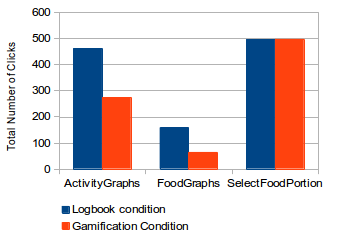
\includegraphics[width=0.6\textwidth]{self_monitoring_usage.png}
    \rule{35em}{0.5pt}
  \caption{Total clicks on feedback features for self-monitoring of wellness: ``Logbook App'' versus ``Gamified App''.}
  \label{figure:self_monitoring_usage}
\end{figure*}\newline
Another important finding on usage showed that the main logbook component functionality such as steps graphs, and diet charts had lower utilization during gamification condition compared to during logbook condition as shown on Figure \ref{figure:self_monitoring_usage}. This happens as intermediary participants paid more focus on virtual rewards which provided indirect feedbacks of steps and diet through badges, gardens etc. This is further supported by Figure \ref{figure:clicks_distr} which shows the distribution of clicks among feedback features of the ``Gamified Wellness App'' and ``The Logbook App''.\newline  However, the trend in recording of diet/meals was almost similar between the two experimental conditions as the process of recording meals was instrumental in earning virtual rewards during gamification condition, therefore, intermediary participants continued to use that feature while in gamification condition. In addition, pairs that had been exposed to gamification condition before logbook condition, showed a sudden drop in number of sessions after being switched to logbook. These users had already used features that are present in logbook condition while they were still in logbook condition hence withdrawing of virtual rewards made them them reduce their app usage by a significant number  as shown on Table.  This finding also explains why usage on Figure \ref{figure:usagedailysessions} above showed a sharp decline of sessions in logbook condition in between the fourth and fifth weeks. This is a period where the switching of experimental conditions happened.\newline
\begin{figure}[htbp]
  \centering
    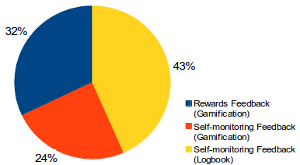
\includegraphics[width=0.45\textwidth]{clicks_distr.png}
    \rule{26em}{0.5pt}
  \caption{Total clicks on feedback features in the two experimental conditions : self-monitoring features versus rewards features.}
  \label{figure:clicks_distr}
\end{figure}\newline
Another important observation showed an indication that more gamification sessions were likely to come from pairs that had young intermediary participants (age \textless Median=15.5 years) as shown on Figure \ref{figure:gambyage}. Intermediaries from both age group were distributed almost evenly to the two experimental sequences, therefore, the relativity of number of sessions doesn't matter on this trend. Also the overall average trend on usage of the app during the six weeks demonstrated an indication of younger intermediaries (age \textless median age) tendency of using the app more often compared  to their older counterparts since more sessions. The trend was still similar after excluding the four pairs (Table \ref{table:usageproblems}) that had usage problems.\newline
\begin{figure}[htbp]
  \centering
    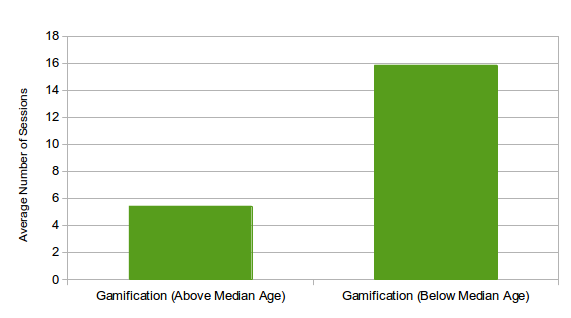
\includegraphics[width=0.4\textwidth]{gambyage.png}
    \rule{26em}{0.5pt}
  \caption{Average number of gamification sessions on  14 pairs by intermediaries' age: Age \textgreater= median age(=15.5) versus Age \textless median age.}
  \label{figure:gambyage}
\end{figure}\newline
\subsection{User Experience}
From the previous, there was an indication of younger intermediaries (age\textless median=15.5 years) to have more number of sessions on average compared to their older counterparts. However, baseline trend on perceived enjoyment to help with cellphone related tasks contradicts this trend as younger intermediaries appear not to be enjoying the task of helping compared to their older counterparts (Figure \ref{figure:PE_HELP_Age}).\newline
\begin{figure}[htbp]
  \centering
    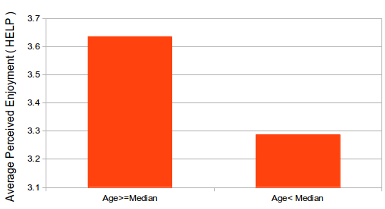
\includegraphics[width=0.35\textwidth]{PE_HELP_Age.png}
    \rule{26em}{0.5pt}
  \caption{Intermediaries' average perceived enjoyment to help others with cellphone tasks versus age group}
  \label{figure:PE_HELP_Age}
\end{figure}

\begin{figure}[htbp]
  \centering
    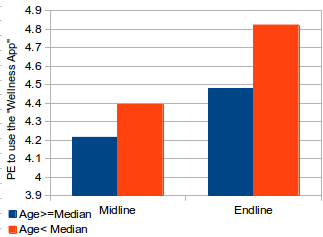
\includegraphics[width=0.35\textwidth]{PE_Interm_App.png}
    \rule{26em}{0.5pt}
  \caption{Intermediaries' average perceived enjoyment in using the app versus age group.}
  \label{figure:PE_Interm_App}
\end{figure}
The trend in younger intermediaries' average perceived enjoyment to use the wellness app (Figure \ref{figure:PE_Interm_App})  appears to be more compared to the older counterparts despite the fact that these younger intermediaries showed less interest at baseline. This trend resonates with aforementioned usage of the app.\newline
There are factors that played an instrumental role in motivating intermediaries to use the app in the two experimental conditions and these factors are regardless of the age group of intermediaries. But some these mediating factors appeared to had more effect on young intermediaries. The first factor was
\emph{\textbf{``self-monitoring task''}}. The task itself of self-monitoring without rewards sparked interests of some intermediary users. This might be as the result of the novelty effect of visualization mechanisms. For instance one intermediary user who happened to be the youngest among all intermediaries reported the highest perceived enjoyment during logbook condition compared to other intermediary users. In addition it seems the phone also had an impact on triggering her interests.\newline
The second factor that influence usage was \emph{\textbf{``informal comparisons''}}. For intermediaries who were close, they did this form of informal comparison especially during the absence of gamification.\newline 
The third usage factor was \emph{\textbf{``gamification rewards and  competitions''}}. Competitions increased the number of times intermediary user checked the app. During interviews, the researcher discovered that in one pair not only the beneficiary participant was using the pedometer, an intermediary was also taking turns to use the pedometer, therefore they were collaborating in accumulating steps. Both an intermediary user and a beneficiary user had discussions of whether the person whose turn it was had walk enough steps. They did this to accumulate more steps than other pairs.\newline
The fourth and the last usage factor was \emph{\textbf{``requests from beneficiary users''}}:There were times where intermediary users engaged with the app only upon receiving requests from beneficiaries.  We observed cases of where intermediary participants autonomy was violated as requests came at the time where intermediary participants were either studying for exams or doing something else and they felt it was not the right time to fulfil those requests. This made intermediary participant to feel that their parents were nagging them.\newline
However, despite higher frequency of usage in gamification condition, the trend on average perceived enjoyment in logbook appears to be higher than in logbook condition for both age groups as shown on Figure \ref{figure:PE_Interm_App_exp_seq} and this is because not all intermediary participants had a positive user experience on utilizing gamification. We observed two factors that contributed  to this. The first factor is that there were pairs that had usage problems as we have seen on Table \ref{table:usageproblems} above. Among these four pairs, the user experience was severely bad in the users from pairs ``A'' and, ``C''.\newline
For pair A the app demotivated the intermediary of this pair because it was not stable  and it was always failing to load. This happened at the beginning of the experiments and as the result this pair terminated their usage after using the app for only two days of which both days were during the gamification condition.\newline
For pair C, the pedometer never transmitted a single reading to the server but this pair continued to use the app throughout the logbook condition. There are several reasons which include the fact that the intermediary user from this pair was close to another intermediary from pair D which also experienced problems with pedometer but not so severe like an intermediary user from Pair C. Therefore, an intermediary user from pair C continued use the app although the steps never got transmitted to the server. However, steps were being displayed as raw numbers on a native pedometer app. The two intermediary participants from pairs C, D shared their progress about steps walked by their respective beneficiary participants. And this happened whenever they met.  This explained why the pedometer problem didn't affect the usage of the app by the intermediary user from pair C. After pair C was switched to gamification, the inability of the pedometer to transmit steps to the server resulted to negative user experience to the intermediary user from this pair. The reason is that steps played a role in achievement of rewards. And this intermediary user had done a lot of efforts with expectations that their pair will be rewarded once switched to gamification condition. This finding about expectations was shared by another intermediary user from pair E who was living close  to the two intermediaries from pairs C, D. She was concerned about the gamification system as she worried that the system was not fair because her peers had done more efforts compared to her but she was ahead of them and she didn't understand why was it the case. She was referring to what she had observed during logbook condition,  therefore she was expecting the efforts of her pears to transmute into rewards after they were both switched to gamification condition.  As the result the problems on pairs C, D had a multiplier  effect on the perceived enjoyment of this intermediary user from pair E hence her motivation to use the gamified app was negatively affected.\newline 
\begin{figure}[htbp]
  \centering
    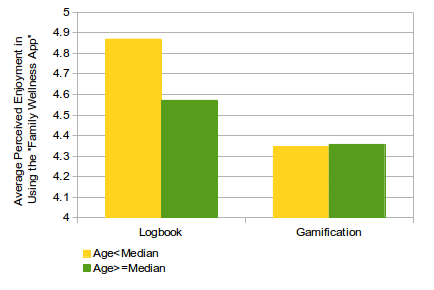
\includegraphics[width=0.5\textwidth]{PE_Interm_App_exp_seq.png}
    \rule{26em}{0.5pt}
  \caption{Intermediaries' average perceived enjoyment in using the app versus age group (Logbook and Gamification).}
  \label{figure:PE_Interm_App_exp_seq}
\end{figure}\newline
Gamification condition didn't harm motivation of only users with severe usability problems (pairs A, C) as there was  a very intriguing phenomenon on two other intermediary users from \textbf{Pair F} and \textbf{Pair G}. The two intermediary users had used the app more often in gamification condition  compared to when they were in logbook condition but had reported both lower scores in perceived enjoyment, and perceived competence when in gamified condition compared to when they were in logbook condition. On reviewing their performance on gamification, it was observed that these two users never attained any advancement in badges despite their efforts during gamification condition. The reason for this is that their beneficiary participants were not walking enough steps despite the fact that these intermediaries had put  more efforts in using the App during gamification condition. Badges were earned in combination of both the app usage and average number of steps walked by a beneficiary user. Therefore the absence of rewards harmed both their interest to use the ``Family Wellness App'' while in gamification condition. We attribute this negative experience to failure of our gamification system to match challenges with abilities. i.e. efforts of beneficiaries differed hence challenges should have matched with individual abilities of beneficiaries within pairs. When challenges are too difficult as they don't match users' skills, end users can become demotivated \cite{zhang2008:motivational}.\newline
We also compared the ability of the two versions of the app to afford the three basic psychological needs. In this comparison we excluded pairs A, C, F, and G due the reasons we have mentioned above. The results for this comparison is shown on Table \ref{table:imiwellnessinterm}.
\begin{table}[h!]
  \begin{center}
    \caption{Comparison of 10 intermediaries' scores on sub-scales of perceived competence (PC), perceived autonomy (PA), and perceived relatedness (PR) in using the ``Family Wellness App}
    \label{table:imiwellnessinterm}
	\begin{tabular}{|c|c|c|}
		\hline
		Mean &Logbook&Gamification\\
		\hline
		 \multirow{2}{*}{PC}&M=5.23; SD=1.02&M=5.96; SD=0.66\\\cline{2-3} 

		 &\multicolumn{2}{|l|}{t(9)=-3.4949; p=0.0068 ; 95\% CI= -1.204 to -0.258} \\
\hline
		 \multirow{2}{*}{PA}&M=3.95; SD=0.86&M=3.96; SD=0.94\\\cline{2-3} 

		 &\multicolumn{2}{|l|}{t(9)= -0.0269; p= 0.9792; 95\% CI= -0.596 to 0.582} \\
\hline

		 \multirow{2}{*}{PR}&M=4.22; SD=0.63&M=4.37; SD=0.9\\\cline{2-3} 
		 &\multicolumn{2}{|l|}{t(9)= -0.7193; p=0.4902; 95\% CI= -0.622 to 0.322 } \\
\hline
	\end{tabular}
  \end{center}
\end{table}
\newline
Perceived competence of intermediaries in using the ``Family Wellness App'' was significantly higher in the gamified condition than in the logbook condition. This means a gamified system gave intermediary users challenges and these challenges motivated an increase in frequency of using the app. There ware no significant difference on both perceived autonomy and relatedness. Perceived autonomy doesn't differ because in both experimental conditions usage was either self-initiated by beneficiary user some of the time but there were also cases of were requests to initiate interaction came from beneficiary participants. perceived relatedness also doesn't differ and the reason for this is most users where already close friends before this intervention hence either versions of the app didn't change anything about how they relate to each other.\newline  
\subsection{User Experience of Beneficiaries} 
Since most beneficiary participants relied on their intermediary participants to access the app it was difficult to assess whether the versions of the prototype fulfil the three basic psychological needs or not. However, we observed situations of where beneficiary had negative experience, especially when they need help and intermediary participants feel they are being bothered. This happened even in gamification especially for users who didn't enjoy gamification.\newline
We also compared the overall impact of the app for self-monitoring at midline and endline with comparison to baseline on motivation to self-monitor diet and activity. We used the IMI questionnaire with six sub-scales; perceive competence, perceived autonomy,perceived relatedness, perceived enjoyment,  perceived usefulness, and perceived effort. The overall IMI score was computed by averaging scores from individual sub-scales.
Only ten beneficiary participants were considered for analysis. Four were excluded because of usage problems highlighted on Table \ref{table:usageproblems} as it affected their ability to self-monitor their wellness.\newline
The first comparison was on self-monitoring of diet at baseline, midline, and endline. I used one way ANOVA with repeated measures. The results on self-monitoring of diet (baseline, midline, and endline) are shown on Table  \ref{table:imidietbenf}.  The Mauchly's test indicated that the assumption of sphericity was not violated with  $\chi{}$\SP{2}(2)=3.76, p=0.152. The ANOVA showed that there was a significant time effect on average IMI scores  to self-monitoring diet measured at baseline, midline and endline. Also pairwise comparisons with a paired student t-test indicated that the average score was significantly higher at endline when compare to baseline (t(9)=-2.457; p=0.036; 95\% CI= -2.06083 to -0.08517 ). There were no significant differences between midline and baseline (t(9)=-1.298; p=0.227 ; 95\% CI= -1.621 to 0.439), and between midline and endline (t(9)=-1.975; p=0.08 ; 95\% CI= -1.0342 to 0.07017). But if we repeat the ANOVA analysis with baseline, logbook and gamification the difference is not significant. However, the trend on averages shows that both gamification and logbook result into an increase of motivation to self-monitor diet as shown on Figure \ref{figure:imi_diet2}\newline
\begin{table}[h!]
  \begin{center}
    \caption{Comparison of ten beneficiaries' IMI scores in self-monitoring of diet at baseline, midline and endline}
    \label{table:imidietbenf}
	\begin{tabular}{|L{3.3cm}|L{1.1cm}|L{1.1cm}|L{1.1cm}|}
		\hline
		Mean IMI Score &Baseline&Midline&Endline\\
		\hline
		 %\multirow{3}{*}
		 {Self-monitoring of Diet}&M=4.48; SD=1.24&M=5.07; SD=1.19;&M=5.55; SD=0.95\\\cline{2-4} 

		&\multicolumn{3}{|l|}{F(2,18)=3.787; p=0.042} \\
\hline	\end{tabular}
  \end{center}
\end{table}\newline
\begin{figure}[htbp]
  \centering
    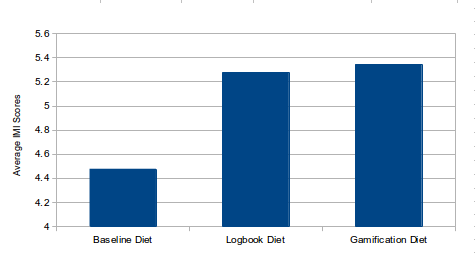
\includegraphics[width=0.4\textwidth]{imi_diet2.png}]
    \rule{26em}{0.5pt}
  \caption{Trend on Average IMI Scores of Self-Monitoring of Diet at Baseline, Logbook, and Gamification.}
  \label{figure:imi_diet2}
\end{figure}
We conducted another analysis (N=9) to examine if there is a difference among baseline,midline, and endline in self-monitoring of activity. The sample size was now 9 because one participant didn't complete the questionnaire. ANOVA (Table \ref{table:imiactivitybenf}) showed that there was no significant difference of average IMI scores on self-monitoring of activity measured at baseline, midline and endline. The trend of means appears to increase from baseline to endline as shown on Figure \ref{figure:imi_activity}.
\begin{table}[h!]
  \begin{center}
    \caption{Comparison of ten beneficiaries' IMI scores in self-monitoring of activity at baseline, midline and endline}
    \label{table:imiactivitybenf}
	\begin{tabular}{|L{2.5cm}|L{1.3cm}|L{1.3cm}|L{1.5cm}|}
		\hline
		Mean IMI Score &Baseline&Midline&Endline\\
		\hline
		 %\multirow{3}{*}
		 Self-monitoring&M=4.82; SD=1.002&M=5.28; SD=1.003&M=5.41; SD=0.894\\\cline{2-4} 
		 of activity&\multicolumn{3}{|l|}{F(1.182, 9.455)=2.936; p=0.116} \\
\hline	\end{tabular}
  \end{center}
\end{table}\newline 
\begin{figure}[htbp]
  \centering
    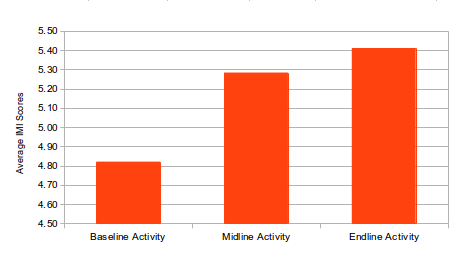
\includegraphics[width=0.4\textwidth]{imi_activity.png}
    \rule{26em}{0.5pt}
  \caption{Trend on Average IMI Scores of Self-Monitoring of Activity at Baseline, Logbook, and Gamification.}
  \label{figure:imi_activity}
\end{figure}\newline
\section{Discussion}
\section{Conclusions}
%\end{document}  % This is where a 'short' article might terminate

%ACKNOWLEDGMENTS are optional 

%\section{Acknowledgments} 

%
% The following two commands are all you need in the
% initial runs of your .tex file to\ref{equation:sizetrees}
% produce the bibliography for the citations in your paper.
%small{
\bibliographystyle{abbrv}
\bibliography{sigproc} %} % sigproc.bib is the name of the Bibliography in this case
% You must have a proper ".bib" file
%  and remember to run:
% latex bibtex latex latex
% to resolve all references
%
% ACM needs 'a single self-contained file'!
%
%APPENDICES are optional
%\balancecolumns

\end{document}
